\documentclass[11pt,a4paper]{article}
\usepackage[utf8]{inputenc}
\usepackage[T1]{fontenc}
\usepackage[french]{babel}
\usepackage{amsmath, amssymb}
\usepackage[margin=2.5cm]{geometry}
\usepackage{graphicx}
\usepackage{hyperref}
\usepackage{titlesec}
\usepackage{parskip}

\title{Hyperpop! \\ \normalsize{Jeu de tir dans un espace en 4D}}
\author{Caio COSTA, Youssef SAIDI}
\date{Printemps 2025}

\begin{document}

\maketitle

\tableofcontents

\section{Introduction}

Ce projet a consisté à concevoir un jeu interactif se déroulant dans un espace à quatre dimensions, où le joueur doit tirer sur des sphères 4D. L’originalité du jeu réside dans le fait que les objets 4D ne sont pas visualisés directement, mais à travers leur intersection avec un hyperplan 3D, que le joueur peut déplacer le long de la quatrième dimension.

Ce travail nous a permis d'explorer les concepts de géométrie en dimension supérieure, tout en les rendant accessibles via une représentation tridimensionnelle interactive et intuitive.

\section{Modélisation géométrique}

\subsection{Sphères en 4D}

Une sphère dans l’espace $\mathbb{R}^4$ est définie comme l’ensemble des points situés à une distance constante $r$ d’un centre $(x_0, y_0, z_0, w_0)$ :
\[
	(x - x_0)^2 + (y - y_0)^2 + (z - z_0)^2 + (w - w_0)^2 = r^2.
\]

\subsection{Hyperplan 3D de visualisation}

Pour visualiser les objets 4D, nous utilisons un hyperplan de la forme $w = c$, avec $c$ variable. Ce plan agit comme une « caméra » 3D qui balaie l’espace 4D et en extrait une coupe tridimensionnelle observable à l’écran.

On peut se représenter ce procédé par analogie avec la 3D : l’intersection d’un cube avec un plan peut donner un point, un triangle, un carré ou un hexagone, selon la position du plan. En revanche, l’intersection d’une sphère donne toujours un disque (ou un cercle). Le même principe s’applique en 4D, ce qui justifie le choix de sphères pour notre jeu.

\begin{figure}[h]
	\centering
	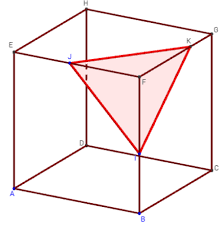
\includegraphics[width=0.3\linewidth]{intersection-cube}
	\caption{Intersection d’un plan avec un cube}
	\label{fig:inter-plan-cube}
\end{figure}

\begin{figure}
	\centering
	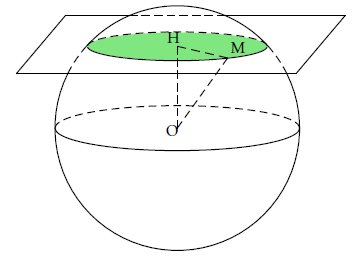
\includegraphics[width=0.3\linewidth]{intersection-sphere}
	\caption{Intersection d’un plan avec une sphère}
	\label{fig:inter-plan-sphere}
\end{figure}

\subsection{Intersection sphère 4D / hyperplan 3D}

L’intersection d’une sphère 4D avec le plan $w = c$ est une sphère 3D (ou vide si le plan est trop éloigné du centre dans la direction $w$). Le rayon de cette coupe est donné par :
\[
	r' = \sqrt{r^2 - (w_0 - c)^2},
\]
à condition que $|w_0 - c| \leq r$.

\section{Mécanique du jeu}

\subsection{Navigation dans la quatrième dimension}

Les objets du jeu sont positionnés dans l’espace via une matrice \textit{model}. Pour simuler une caméra mobile en 4D, on applique à cette matrice des transformations inverses (translations, rotations), déclenchées par les actions du joueur.

Celui-ci peut se déplacer dans l’espace 3D, mais aussi déplacer l’hyperplan de visualisation dans la direction $w$, révélant ainsi de nouveaux objets.

\subsection{Déplacement des sphères}

Chaque sphère se déplace de manière périodique selon une direction aléatoire déterminée lors de son apparition. Cela crée un environnement dynamique et rend le jeu plus immersif.

\subsection{Système de tir}

Le joueur dispose d’un viseur fixe, centré à l’écran, et peut tirer sur les sphères visibles. En fonction de la sphère touchée, un certain nombre de points est attribué et un effet sonore est joué pour signaler un tir réussi.

\section{Affichage et rendu}

\subsection{Chunks}

Afin de gérer efficacement un espace potentiellement vaste, nous avons découpé l’univers en « chunks », c’est-à-dire en sous-espaces 3D localisés. Seuls les chunks proches de la position actuelle du joueur sont affichés, réduisant ainsi la charge de calcul.

\subsection{Mise à jour par frame}

À chaque image (frame), le moteur de jeu effectue les opérations suivantes :
\begin{itemize}
	\item Lecture des entrées clavier et mise à jour de la matrice \textit{model}.
	\item Détermination des chunks visibles.
	\item Rendu du fond spatial et des étoiles.
	\item Mise à jour des positions des sphères et affichage de leur intersection avec l’hyperplan courant.
\end{itemize}

\subsection{Rendu visuel}

Le rendu est assuré par la bibliothèque \texttt{p5.js}. Les sphères issues des intersections 4D–3D sont affichées comme des sphères 3D classiques. L’ensemble est rendu sur un fond sombre, agrémenté d’étoiles pour renforcer l’ambiance spatiale.

\section{Difficultés rencontrées}

Ce projet a soulevé plusieurs défis, notamment :
\begin{itemize}
	\item \textbf{Projection 4D $\rightarrow$ 3D} : comprendre et implémenter la coupe d’une sphère 4D par un hyperplan.
	\item \textbf{Navigation intuitive} : concevoir des contrôles fluides dans un espace à quatre dimensions.
	\item \textbf{Performance} : maintenir une fluidité satisfaisante malgré un grand nombre d’objets grâce aux chunks.
	\item \textbf{Compatibilité clavier} : gérer les différences entre claviers QWERTY et AZERTY.
\end{itemize}

\section{Perspectives et améliorations}

Afin d’enrichir l’expérience de jeu et d’explorer de nouvelles possibilités, plusieurs axes d’amélioration peuvent être envisagés pour la suite du projet.

\subsection{Nouveaux modes de jeu}

Il serait intéressant d’ajouter différents modes de jeu, tels qu’un mode contre-la-montre où le joueur doit atteindre un score dans un temps limité, ou un mode survie dans lequel la difficulté augmente progressivement. Par exemple, dans un mode « combo », le joueur pourrait obtenir des multiplicateurs de points en touchant plusieurs sphères en un seul tir ou en un court laps de temps.

\subsection{Extension des objets et de la visualisation}

L’introduction d’autres objets 4D, comme des tesseracts ou des polytopes réguliers, permettrait de diversifier les formes rencontrées et d’offrir de nouveaux défis de visualisation. De plus, proposer une visualisation alternative, par exemple via une projection perspective depuis la 4D, offrirait une nouvelle manière d’appréhender la géométrie de l’espace.

\subsection{Accessibilité et pédagogie}

Pour faciliter la prise en main, un tutoriel interactif pourrait guider le joueur dans la navigation en 4D et l’utilisation des contrôles. Des explications visuelles ou des animations pédagogiques pourraient également aider à comprendre les principes de l’intersection et de la projection.

\subsection{Effets visuels et ambiance}

L’ajout d’effets visuels, tels que des explosions, des particules ou des bulles éclatantes lors des impacts, renforcerait l’immersion et le plaisir de jeu. De même, remplacer la lumière fixe en 3D par une lumière dynamique en 4D, cohérente avec la position du joueur, permettrait d’obtenir un rendu plus réaliste et spectaculaire.

\subsection{Portage mobile}

Enfin, développer une version mobile du jeu permettrait de toucher un public plus large. Cependant, cela impliquerait une refonte complète de l’interface et des contrôles pour s’adapter aux écrans tactiles, ce qui représenterait un travail conséquent et nécessiterait beaucoup plus de temps de développement.

\section{Ressources et accès au projet}

Le code source, la documentation et une version jouable du projet sont disponibles en ligne :
\begin{itemize}
    \item \textbf{Page GitHub} : \url{https://github.com/bissectra/hyperpop}
    \item \textbf{Jouer en ligne} : \url{https://bissectra.github.io/hyperpop/}
\end{itemize}

La gestion du projet a été assurée à l'aide de \textbf{Git} pour le suivi des versions et de la plateforme \textbf{GitHub} (issues, pull requests) pour organiser les tâches, suivre les bugs et coordonner le travail collaboratif.

\section{Conclusion}

Ce projet a été l’occasion d’aborder de manière concrète et ludique les enjeux de la visualisation en dimension supérieure. Il nous a permis de mobiliser des compétences en géométrie, en programmation graphique et en conception interactive pour créer une expérience originale, immersive et pédagogique.

\end{document}